%\minote{This is working..}
\section*{Appendix}
\label{sec:appendix}
\section{Examples of insecure patterns in code snippets}

\begin{lstlisting}[caption={A code snippet showing insecure use of AES default encryption mode ECB.}, label={fig:aes-encryption-example}]
    private byte[] encrypt(byte[] raw, byte[] clear) {
      ...
      Cipher cipher = Cipher.getInstance("AES");}
      ....
      return encrypted
    }
     \end{lstlisting}

\begin{lstlisting}[caption={A code snippet showing insecure use of Absence of performing hostname verification.}, 
label={listing:Absence-of-performing-hostname-verification}]
   public static void allowAllSSL() {
            HttpsURLConnection.setDefaultHostnameVerifier(new HostnameVerifier() {

                @Override
                public boolean verify(final String hostname, final SSLSession session) {
                    return true;
                }
            });
      ...
   }
\end{lstlisting}

\begin{lstlisting}[caption={A code snippet showing insecure use of weak key length.}, 
label={listing:Weak-key-length}]

public byte[] RSAEncrypt(final String plain) throws ... {
    kpg = KeyPairGenerator.getInstance("RSA");
    kpg.initialize(1024);
    kp = kpg.genKeyPair();
    publicKey = kp.getPublic();
    privateKey = kp.getPrivate();

    cipher = Cipher.getInstance("RSA");
    ... 
}
\end{lstlisting}

\begin{lstlisting}[caption={A code snippet showing insecure use of static predictable IV.}, 
label={listing:Static-constant-predictable-keys-IV}]
    ...
    byte[] salt = "abababababababababa bab".getBytes();
    byte[] iv = "1234567890abcdef".getBytes();
    ... 
}
\end{lstlisting}

\begin{lstlisting}[caption={A code snippet showing insecure use of AllHostNameVerifier.}, 
label={listing:AllHostNameVerifier}]
    ...
    public ServiceConnectionSE(String url) throws IOException {
      ...
      ((HttpsURLConnection) connection).setHostnameVerifier(new AllowAllHostnameVerifier());
      ...
    } 
}
\end{lstlisting}

\begin{lstlisting}[caption={A code snippet showing insecure use of turning off CSRF protection.}, 
label={listing:csrf-protection}]
    ...
    @Override
    protected void configure(HttpSecurity hs) throws Exception {
      hs.csrf.disable()
    }
    ...
\end{lstlisting}





%=============================================================================================================
\iffalse
\begin{lstlisting}[caption={A real code snippet taken from Stackoverflow. I want to build a tool which after analyzing the code snippet will highlight the part of the code that is insecure and suggest an alternative secure implementation as showed in the figure.}, label={fig:motivating-example}]
static void decrypt() {
    ...
    String MyDifficultPassw = "MyDifficultPassw";
    ...  
    SecretKeySpec sks = new SecretKeySpec(MyDifficultPassw.getBytes(), "AES");
    ...
}
\end{lstlisting}
\begin{lstlisting}[caption={A real code snippet taken from Stackoverflow. I want to build a tool which after analyzing the code snippet will highlight the part of the code that is insecure and suggest an alternative secure implementation as showed in the figure.}, label={fig:motivating-example}]
    private byte[] encrypt(byte[] raw, byte[] clear) {
      ...
      MessageDigest md = MessageDigest.getInstance("MD5");
      ....
      return encrypted
    }
\end{lstlisting}



\begin{lstlisting}[caption={A code snippet showing insecure use of AES default encryption mode ECB.}, 
label={fig:aes-encryption-example}]
    private byte[] encrypt(byte[] raw, byte[] clear) {
      ...
      CIPHER_MODE = "AES"
      Cipher cipher = Cipher.getInstance(CIPHER_MODE);}
      ....
      return encrypted
    }
\end{lstlisting}
\fi
%=======================================================================================================================================
\section{Failure to detect abuse of X509TrustManager Verifier interface insecure pattern}
\label{appendix:X509TrustManager}
Unfortunately we were unable to detect insecure use of X509Trust\-Manager. 
According to our understanding, this is because X509Trust\-Manager is written as
annonymous class in the code snippets by developers. PPA can not properly express 
the  annonymous class in Jimple form. We refer the reader to consult Figure~\ref{fig:trustmanager} 
where \texttt{FakeX509TrustManager} class is declared  as annonymous class,  
and it corresponding jimple represention~\ref{fig:trustmanager-jimple} where
\texttt{FakeX509TrustManager} is delcared as phantom class. 
This means it is class for which PPA can not find the implementation.
Subsecquent use of \texttt{FakeX509Trust\-Manager} are replaced by MAGICCLASS hence.

This can be either of the  following two reasons:
\begin{itemize}  
\item Jimple grammer is simple, and can not express Annoymous class.
\item PPA is built on top of a old version of soot 2.2.4 and Java 1.4. The current version of Soot is 4.2.1 which runs on Java 1.9. 
As PPA depends on an outdatet version of Soot and Java, it may cause the problem of not being able to express Annoymous class in Jimple format.
\end{itemize}   
\begin{figure*}[t]
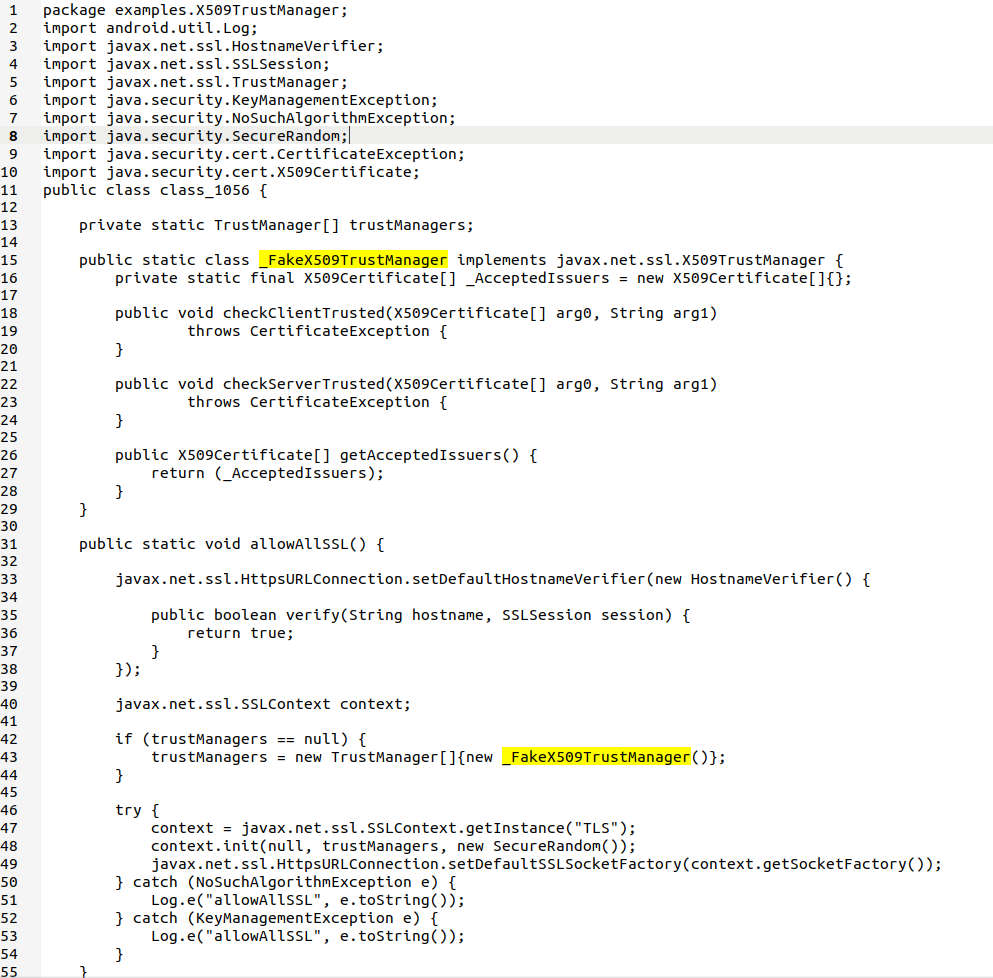
\includegraphics[width=\linewidth]{Figures/Java_TrustManager.png}
\caption{An example of insecure X509TrustManager implementation which we have not been able to detect. 
Corresponding Jimple representation is show in Figure~\ref{fig:trustmanager-jimple} }
\label{fig:trustmanager}
\end{figure*}
\begin{figure*}[t]
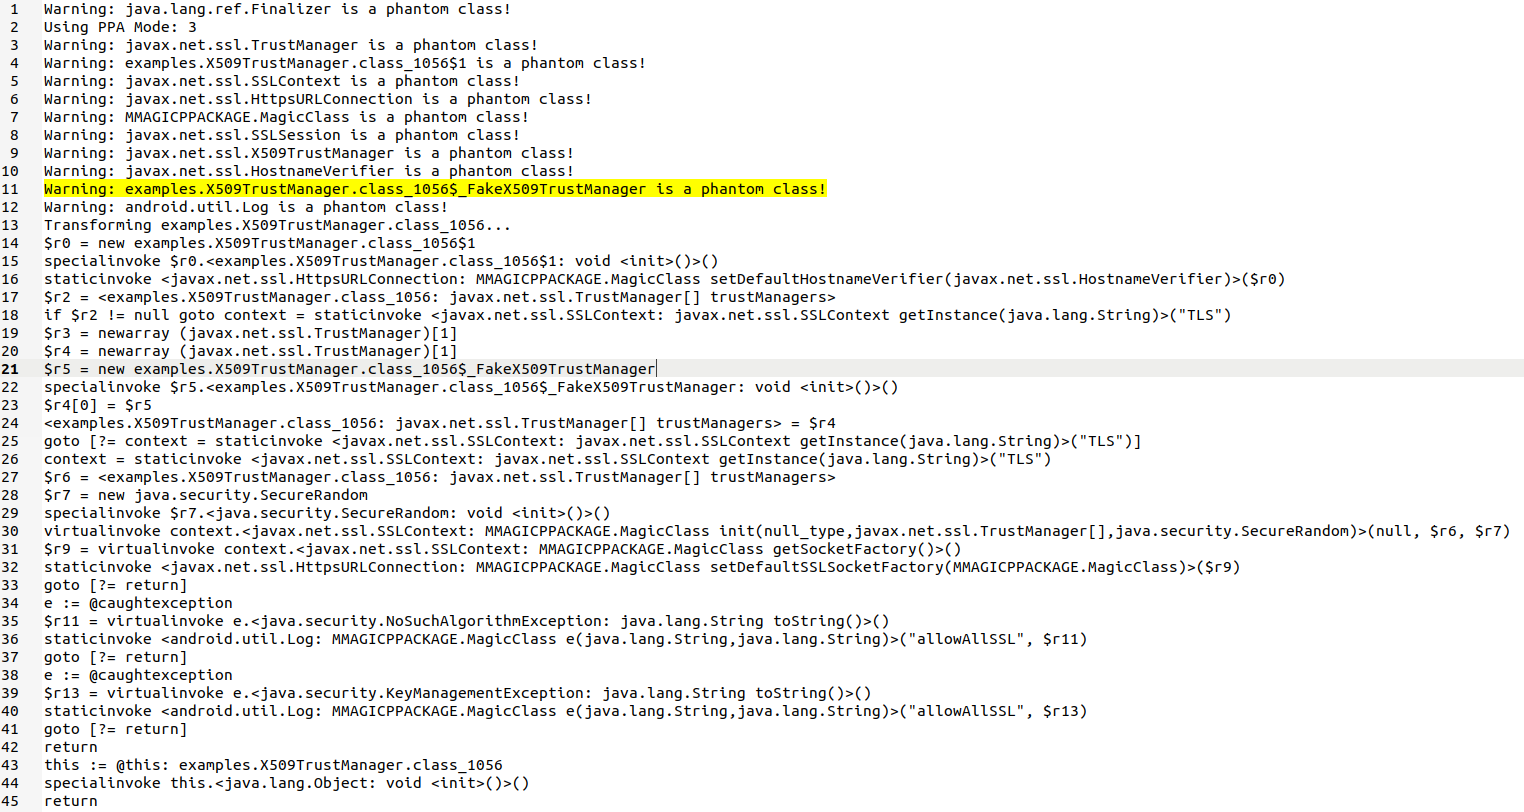
\includegraphics[width=\linewidth]{Figures/Jimple_TrustManager.png}
\caption{Jimple represention of the code snippets in Figure~\ref{fig:trustmanager}. The interesting part is \texttt{\_FakeX509TrustManager} is declared as phantom class (highlighted in yellow color).}
\label{fig:trustmanager-jimple}
\end{figure*}

\section{Future work on Synthesizing secure code}
\section{Links to source files}
\begin{itemize}
\item source code: \url{https://github.com/islamazhar/Detecting-Insecure-Implementation-code-snippets/tree/master/PPA}
\item Data set of all code snippet: \url{https://github.com/islamazhar/Detecting-Insecure-Implementation-code-snippets/tree/master/PPA/src/examples}
\end{itemize}
